\documentclass[12pt,a4paper]{article}
\usepackage{fontspec}
\setmainfont{Times New Roman}
\setsansfont{Arial}
\setmonofont{Courier New}
\usepackage[provide=*,english,romanian]{babel}
\usepackage{amsmath,amssymb,graphicx,geometry,setspace}
\usepackage{fancyhdr,caption,float,listings,xcolor,booktabs,longtable,array,calc}
\usepackage{subcaption,etoolbox,upquote}
\usepackage[unicode,hidelinks]{hyperref}
\geometry{top=2cm,bottom=2cm,left=2.5cm,right=2.5cm}
\setstretch{1.5}
\setlength{\parindent}{0pt}
\setlength{\parskip}{5pt}
\makeatletter
\renewcommand\section{\@startsection{section}{1}{0pt}{16pt}{7pt}{\normalfont\Large\bfseries}}
\renewcommand\subsection{\@startsection{subsection}{2}{0pt}{12pt}{5pt}{\normalfont\large\bfseries}}
\renewcommand\subsubsection{\@startsection{subsubsection}{3}{0pt}{9pt}{4pt}{\normalfont\normalsize\bfseries}}
\makeatother
\setcounter{secnumdepth}{-1}
\pagestyle{fancy}
\fancyhf{}
\rfoot{\thepage}
\renewcommand{\headrulewidth}{0pt}
\setlength{\headheight}{15pt}
\captionsetup{font=small,labelfont=bf,skip=6pt,justification=raggedright,singlelinecheck=false}
\captionsetup[figure]{position=above}
\lstset{language=C,basicstyle=\ttfamily\fontsize{9.5}{11.5}\selectfont,
  columns=fullflexible,showstringspaces=false,tabsize=2,numbersep=8pt,
  frame=single,rulecolor=\color{black!35},breaklines=true,keepspaces=true,
  xleftmargin=4pt,xrightmargin=4pt,aboveskip=8pt,belowskip=8pt}
\AtBeginEnvironment{lstlisting}{\singlespacing}
\AtBeginEnvironment{longtable}{\small\singlespacing}
\setlength{\emergencystretch}{3em}
\providecommand{\tightlist}{\setlength{\itemsep}{0pt}\setlength{\parskip}{0pt}}
\providecommand{\passthrough}[1]{#1}
\providecommand{\pandocbounded}[1]{#1}
\hypersetup{pdftitle={Sisteme de operare — Laborator 12},pdfauthor={Tacu Igor}}
\clubpenalty=10000
\widowpenalty=10000
\displaywidowpenalty=10000
\begin{document}
\begin{titlepage}
\thispagestyle{empty}
\begin{center}
\setstretch{1.18}

\includegraphics[width=0.23\textwidth]{scripts/report-style/utm-logo.png}\\[12pt]
\textbf{MINISTERUL EDUCAȚIEI ȘI CERCETĂRII}\\
\textbf{AL REPUBLICII MOLDOVA}\\[4pt]
\textbf{Universitatea Tehnică a Moldovei}\\
\textbf{Facultatea de Calculatoare, Informatică și Microelectronică}\\
\textbf{Departamentul Inginerie Software și Automatică}\\[36pt]
{\fontsize{22}{26}\selectfont\textbf{Raport}}\\[10pt]
Lucrare de laborator nr. 12\\[8pt]
\textbf{\large Sisteme de operare}\\[24pt]
\textbf{Tema:} Producător–consumator, variabile de condiție, cititori–scriitori și deadlock
\end{center}
\vfill
\begin{flushright}
\setstretch{1.25}
Realizat de:\\
stud. gr. FAF-242, Tacu Igor\\[24pt]
Verificat de:\\
Reițman Patricia
\end{flushright}
\vfill
\begin{center}\textbf{Chișinău – 2026 }\end{center}
\end{titlepage}

\setcounter{page}{1}
\section{Scopul lucrării}\label{scopul-lucrux103rii}

Combinarea primitivelor de sincronizare pentru transfer FIFO,
notificarea unei condiții, acces partajat la date și prevenirea
așteptării circulare.

\section{Sarcina lucrării}\label{sarcina-lucrux103rii}

\begin{itemize}
\tightlist
\item
  Verificarea bufferului de patru elemente și reproducerea blocajului cu
  ordinea greșită a așteptărilor.
\item
  Compararea așteptării pe condiție cu while și if și explicarea
  re-verificării predicatului.
\item
  Executarea soluției cititori--scriitori și analiza starvation.
\item
  Reproducerea deadlock-ului, repararea ordinii mutexurilor și zece
  rulări fără pauzele deliberate.
\end{itemize}

\section{Considerații teoretice}\label{consideraux21bii-teoretice}

Semafoarele unui buffer limitează sloturile libere și ocupate, iar
mutexul protejează structura. O variabilă de condiție notifică
schimbarea unei stări păstrate separat și verificate sub mutex. Politica
cititori--scriitori stabilește cine poate partaja resursa. Achiziția
mutexurilor în ordine opusă poate produce un ciclu de așteptare; o
ordine comună elimină acel ciclu pentru protocolul testat.

\section{Implementare. Rezultate
practice}\label{implementare.-rezultate-practice}

\subsection{Environment and execution
record}\label{environment-and-execution-record}

The four experiments were compiled and run on the Ubuntu server on 16
November 2026: Linux 6.8.0-142-generic, x86\_64, GCC 13.3.0. The
Makefile uses
{\ttfamily\fontsize{10}{12}\selectfont -std=c11 -Wall -Wextra -O0 -pthread}.
All four submitted programs and the four experimental variants compiled
without diagnostics. The actual commands, outputs, exit codes and source
checksums are retained in
\href{https://github.com/igortacu/OS/blob/main/Lab12/evidence/execution.txt}{execution.txt};
\href{https://github.com/igortacu/OS/blob/main/Lab12/evidence/results.json}{results.json}
records the checked results.

The programs follow the Lab 12 handout. Unused thread arguments are
marked, thread IDs use stable per-thread storage, and synchronization
objects are destroyed after joins.
{\ttfamily\fontsize{10}{12}\selectfont \_DEFAULT\_SOU\allowbreak{}RCE}
exposes {\ttfamily\fontsize{10}{12}\selectfont usleep} with the selected
C dialect on glibc. Output is line-buffered in the two programs
deliberately used for timeout experiments, so the record retains their
diagnostic lines. These teaching examples assume successful thread
creation and synchronization initialization, as in the handout.

Two details were corrected:
{\ttfamily\fontsize{10}{12}\selectfont readers.c} prints the shared
reader count while holding
{\ttfamily\fontsize{10}{12}\selectfont rlock}, and the fixed
{\ttfamily\fontsize{10}{12}\selectfont deadlock.c} describes the actual
A-then-B lock order in its messages. The original incorrect variants are
generated separately by
\href{https://github.com/igortacu/OS/blob/main/Lab12/prepare-variants.py}{prepare-variants.py};
they do not overwrite the submitted programs.

\subsection{Part 1 --- Producer and
consumer}\label{part-1-producer-and-consumer}

Source:
\href{https://github.com/igortacu/OS/blob/main/Lab12/prodcons.c}{prodcons.c}.
The circular buffer has four slots and transfers items 1 through 8.
{\ttfamily\fontsize{10}{12}\selectfont empty} starts at 4,
{\ttfamily\fontsize{10}{12}\selectfont full} starts at 0, and the mutex
protects the buffer, indices and diagnostic count.

\par\noindent\begin{minipage}{\linewidth}

\begin{lstlisting}[language=C]
sem_wait(&empty);
pthread_mutex_lock(&lock);
buf[in] = item;
in = (in + 1) % SIZE;
count++;
printf("put %d (in buffer: %d)\n", item, count);
pthread_mutex_unlock(&lock);
sem_post(&full);
\end{lstlisting}

\end{minipage}\par

The saved run reached occupancy 4, consumed all eight items in order,
and finished at zero. The automated check reconstructs the queue from
all 16 events. It verifies every printed occupancy against the
reconstructed queue, checks the range 0--4, and checks that each item is
put and taken once in FIFO order. The complete output is in
\href{https://github.com/igortacu/OS/blob/main/Lab12/evidence/prodcons.txt}{prodcons.txt}.

\textbf{1. Which call stops the producer?}
{\ttfamily\fontsize{10}{12}\selectfont sem\_wait(\&em\allowbreak{}pty)}
blocks when no free-slot permit remains. A successful wait reserves one
slot before the producer touches the buffer. The consumer returns that
permit with
{\ttfamily\fontsize{10}{12}\selectfont sem\_post(\&em\allowbreak{}pty)}
after removing an item. This follows the documented blocking behavior of
\href{https://man7.org/linux/man-pages/man3/sem_wait.3.html}{sem\_wait}.

\textbf{2. Who waits initially?} If the consumer runs before any item is
published, it waits in
{\ttfamily\fontsize{10}{12}\selectfont sem\_wait(\&fu\allowbreak{}ll)}
because {\ttfamily\fontsize{10}{12}\selectfont full} is initially zero.
The producer initially has four empty-slot permits. Starting the
consumer thread first does not guarantee the scheduler will execute it
first; it could reach its wait after the producer has already posted an
item.

\textbf{3. Lock the mutex before waiting for an empty slot.} The
separate
{\ttfamily\fontsize{10}{12}\selectfont variants/pro\allowbreak{}dcons\_bad}
run printed puts 1--4 and then stopped making progress;
{\ttfamily\fontsize{10}{12}\selectfont timeout -k 1 5} returned 124.
When the buffer is full, the producer can hold the mutex while waiting
for {\ttfamily\fontsize{10}{12}\selectfont empty}. The consumer needs
that mutex to remove an item and post
{\ttfamily\fontsize{10}{12}\selectfont empty}. Neither can release the
resource the other needs:

\par\noindent\begin{minipage}{\linewidth}

\begin{lstlisting}
producer holds lock -> waits for an empty slot
consumer needs lock -> cannot remove an item -> cannot return an empty slot
\end{lstlisting}

\end{minipage}\par

The submitted version retains the correct order: reserve a slot first,
then acquire the mutex. A timeout alone is only evidence of
non-completion; the source and the full-buffer state explain the
deadlock in this experiment.

\subsubsection{Native Terminal evidence --- bounded FIFO
transfer}\label{native-terminal-evidence-bounded-fifo-transfer}

\par\medskip\noindent\begin{minipage}{\linewidth}\setstretch{1.0}
\captionof*{figure}{Figura 1. Native Terminal capture: build of all four programs and the complete producer–consumer execution.}
\centering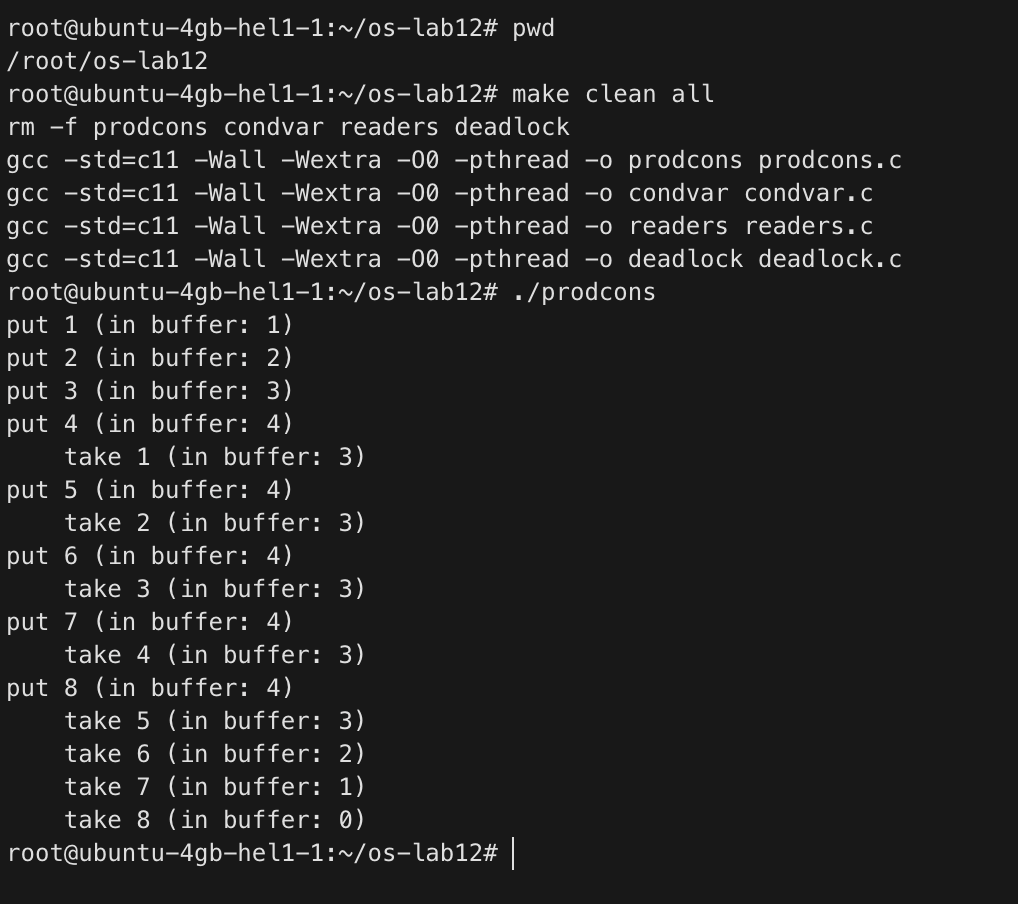
\includegraphics[width=\linewidth,height=0.67\textheight,keepaspectratio]{Lab12/evidence/screenshots/lab12-prodcons-terminal.png}
\end{minipage}\par\medskip

The interactive capture shows the working directory
{\ttfamily\fontsize{10}{12}\selectfont /root/os-lab\allowbreak{}12} and
all four programs compiling with
{\ttfamily\fontsize{10}{12}\selectfont -std=c11 -Wall -Wextra -O0 -pthread},
without compiler diagnostics. The producer inserts items 1--8, and the
consumer removes them in the same order. The printed occupancy reaches
four, stays within zero to four throughout the 16 events, and ends at
zero after item 8 is consumed. This is a live repeat run, separate from
the saved scripted execution.

\subsubsection{Native Terminal evidence --- incorrect producer lock
order}\label{native-terminal-evidence-incorrect-producer-lock-order}

\par\medskip\noindent\begin{minipage}{\linewidth}\setstretch{1.0}
\captionof*{figure}{Figura 2. Native Terminal capture: variant generation, incorrect producer lock order, full buffer and timeout exit code 124.}
\centering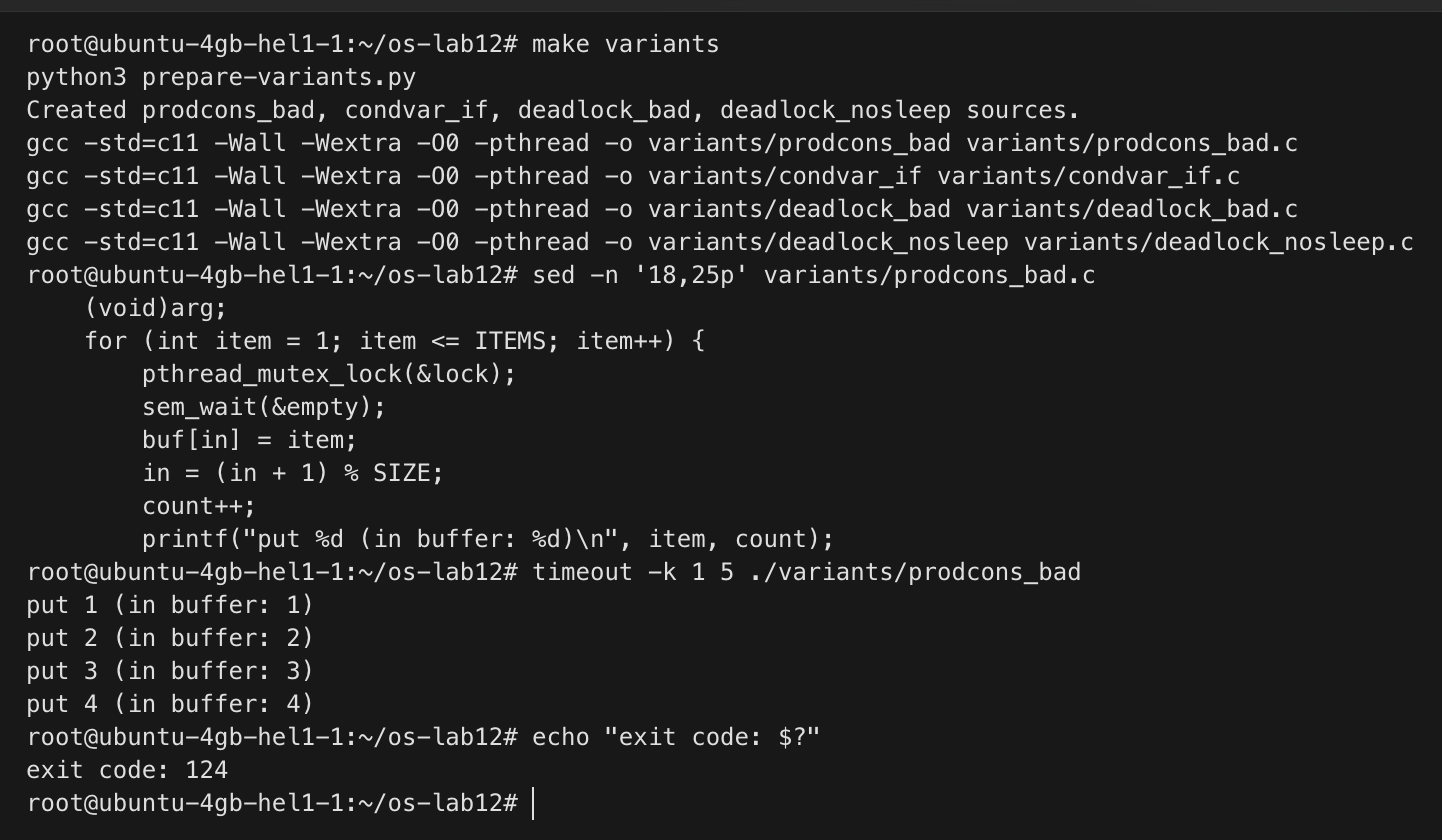
\includegraphics[width=\linewidth,height=0.67\textheight,keepaspectratio]{Lab12/evidence/screenshots/lab12-prodcons-deadlock-terminal.png}
\end{minipage}\par\medskip

The source excerpt places
{\ttfamily\fontsize{10}{12}\selectfont pthread\_mute\allowbreak{}x\_lock(\&lock\allowbreak{})}
before
{\ttfamily\fontsize{10}{12}\selectfont sem\_wait(\&em\allowbreak{}pty)}.
The repeat run prints only puts 1--4, reaching occupancy four, and is
terminated by the five-second timeout with exit code 124. No take is
printed. Together with the inspected source, this supports the
full-buffer deadlock: the producer waits for a free-slot permit while
holding the mutex, preventing the consumer from removing an item and
returning a permit. The correct submitted
{\ttfamily\fontsize{10}{12}\selectfont prodcons.c} remains unchanged.

\subsection{Part 2 --- Condition
variable}\label{part-2-condition-variable}

Source:
\href{https://github.com/igortacu/OS/blob/main/Lab12/condvar.c}{condvar.c}.

\par\noindent\begin{minipage}{\linewidth}

\begin{lstlisting}[language=C]
pthread_mutex_lock(&lock);
while (!ready) {
    printf("B: not ready, I sleep\n");
    pthread_cond_wait(&changed, &lock);
}
printf("B: I read \"%s\"\n", message);
pthread_mutex_unlock(&lock);
\end{lstlisting}

\end{minipage}\par

The saved run produced:

\par\noindent\begin{minipage}{\linewidth}

\begin{lstlisting}
B: not ready, I sleep
A: message written
B: I read "hello"
\end{lstlisting}

\end{minipage}\par

\textbf{1. What remembers readiness?} The integer
{\ttfamily\fontsize{10}{12}\selectfont ready}, accessed under the mutex,
remembers the state. The condition variable is a notification mechanism,
not a stored permit. If A finishes first, B sees
{\ttfamily\fontsize{10}{12}\selectfont ready == 1} and does not need an
earlier signal to have been saved.

\textbf{2. Replace {\ttfamily\fontsize{10}{12}\selectfont while} with
{\ttfamily\fontsize{10}{12}\selectfont if}.} The separate
{\ttfamily\fontsize{10}{12}\selectfont variants/con\allowbreak{}dvar\_if}
run also printed the three lines above and exited with zero. With one
reader, one writer and no observed premature wakeup, this run did not
expose the defect. Passing this experiment does not establish that
{\ttfamily\fontsize{10}{12}\selectfont if} is correct.

\textbf{3. Why use {\ttfamily\fontsize{10}{12}\selectfont while}?} A
condition wait may return after a spurious wakeup even though
{\ttfamily\fontsize{10}{12}\selectfont ready} is still zero. B must
recheck the predicate under the mutex and wait again if necessary. The
wait atomically releases the mutex while blocking and reacquires it
before returning, allowing A to acquire the mutex and publish the state.
These semantics and the need to re-evaluate the predicate are specified
in the
\href{https://man7.org/linux/man-pages/man3/pthread_cond_wait.3p.html}{POSIX
condition-wait documentation}. In a more general reusable-resource
example, another awakened thread can also consume the resource before a
waiter reacquires the mutex.

\subsubsection{Native Terminal evidence --- condition wait with while
and if}\label{native-terminal-evidence-condition-wait-with-while-and-if}

\par\medskip\noindent\begin{minipage}{\linewidth}\setstretch{1.0}
\captionof*{figure}{Figura 3. Native Terminal capture: readiness predicate, condition signal and wait, and the while-versus-if repeat runs.}
\centering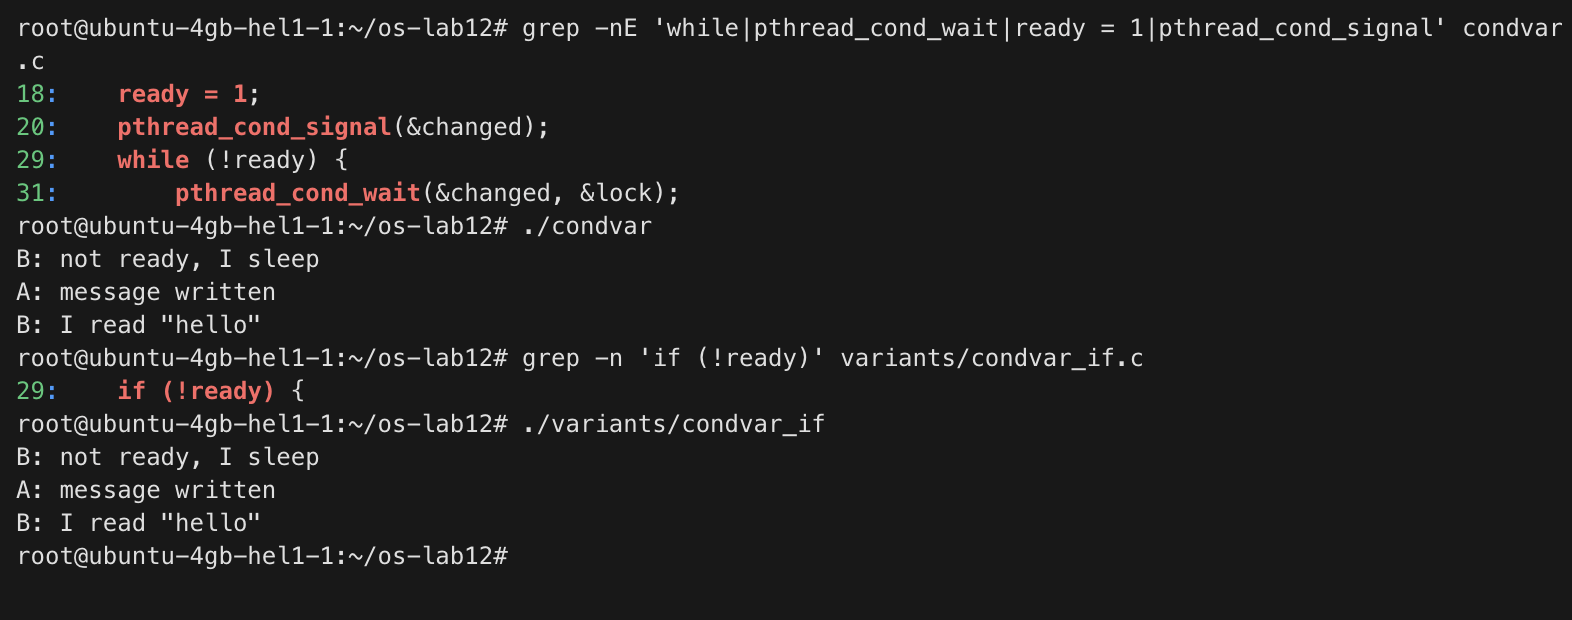
\includegraphics[width=\linewidth,height=0.67\textheight,keepaspectratio]{Lab12/evidence/screenshots/lab12-condvar-terminal.png}
\end{minipage}\par\medskip

The inspected correct source shows
{\ttfamily\fontsize{10}{12}\selectfont ready = 1},
{\ttfamily\fontsize{10}{12}\selectfont pthread\_cond\allowbreak{}\_signal},
and the wait inside
{\ttfamily\fontsize{10}{12}\selectfont while (!ready)}. Its output shows
B sleeping, A writing, and B reading ``hello''. The separate variant
visibly uses {\ttfamily\fontsize{10}{12}\selectfont if (!ready)} and
produces the same three output lines in this repeat run. No premature
wakeup is exposed by this observation, so the successful if run does not
establish general correctness. The submitted
{\ttfamily\fontsize{10}{12}\selectfont condvar.c} retains the while loop
to recheck readiness after every return from the wait.

\subsection{Part 3 --- Readers and
writers}\label{part-3-readers-and-writers}

Source:
\href{https://github.com/igortacu/OS/blob/main/Lab12/readers.c}{readers.c}.
Three readers may overlap; each of the two writers must exclude both
readers and the other writer.

\par\noindent\begin{minipage}{\linewidth}

\begin{lstlisting}[language=C]
sem_wait(&rlock);
if (++readers == 1)
    sem_wait(&room);
printf("reader %ld reads %d (readers inside: %d)\n", id, value, readers);
sem_post(&rlock);
/* Reading interval. */
sem_wait(&rlock);
if (--readers == 0)
    sem_post(&room);
sem_post(&rlock);
\end{lstlisting}

\end{minipage}\par

In all three recorded runs, writer 1 wrote 10, the readers printed 10
with reader counts 1, 2 and 3, then writer 2 wrote 20. The final state
was
{\ttfamily\fontsize{10}{12}\selectfont final value: 20; readers inside: 0}.
The checker verifies the five participant IDs, both increments, the
reader-count range and the final state. These output checks support the
observed run; they are not an exhaustive proof over thread schedules,
and creation order is not a promised execution order.

\textbf{1. Which reader operations allow sharing and exclude writers?}
The first reader executes
{\ttfamily\fontsize{10}{12}\selectfont if (++readers == 1) sem\_wait(\&ro\allowbreak{}om)},
and the last departing reader executes
{\ttfamily\fontsize{10}{12}\selectfont if (--readers == 0) sem\_post(\&ro\allowbreak{}om)}.
The group retains the room permit while readers remain. Later readers
join that group without each acquiring
{\ttfamily\fontsize{10}{12}\selectfont room}; writers must acquire it
individually.

\textbf{2. Why protect {\ttfamily\fontsize{10}{12}\selectfont readers}
with {\ttfamily\fontsize{10}{12}\selectfont rlock}?} Increment,
decrement and the first/last tests must be coordinated. Without
protection, concurrent updates can be lost, two threads can misidentify
the first reader, or the room can be released at the wrong time. The
printed access also needs protection: in the handout it appears after
releasing {\ttfamily\fontsize{10}{12}\selectfont rlock}, where another
reader can modify the count concurrently. This version keeps the print
inside the counter critical section. The subsequent reading intervals
still overlap after {\ttfamily\fontsize{10}{12}\selectfont rlock} is
released.

\textbf{3. What if readers continuously arrive?} This is a
reader-preference algorithm. As long as new readers join before the last
current reader leaves, the group keeps the room permit and a writer can
wait indefinitely: writer starvation. The finite three-reader run does
not demonstrate starvation; it illustrates the policy whose limitation
becomes relevant with a continuing stream of readers.

\subsubsection{Native Terminal evidence --- readers and
writers}\label{native-terminal-evidence-readers-and-writers}

\par\medskip\noindent\begin{minipage}{\linewidth}\setstretch{1.0}
\captionof*{figure}{Figura 4. Native Terminal capture: first-reader and last-reader protocol, protected diagnostic count, and the complete readers–writers execution.}
\centering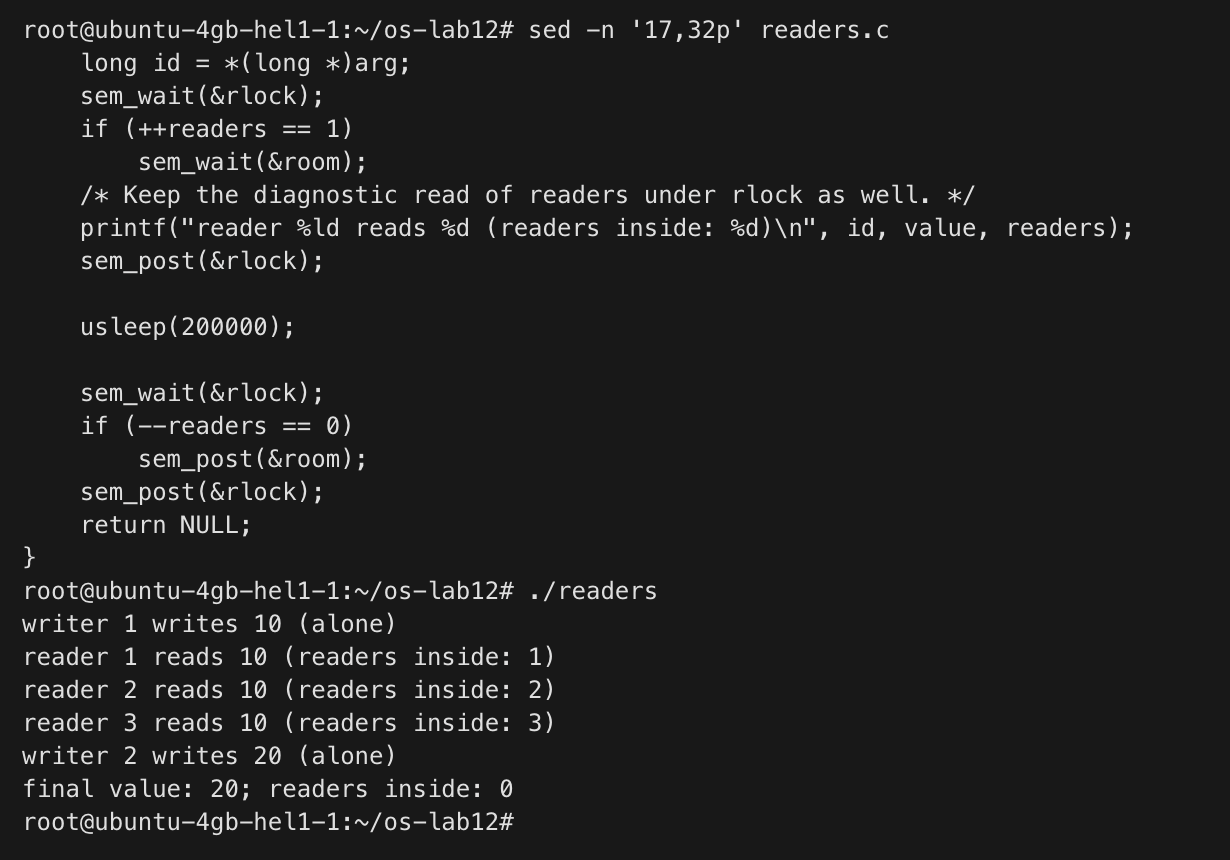
\includegraphics[width=\linewidth,height=0.67\textheight,keepaspectratio]{Lab12/evidence/screenshots/lab12-readers-terminal.png}
\end{minipage}\par\medskip

The inspected source protects the reader counter and its diagnostic
print with {\ttfamily\fontsize{10}{12}\selectfont rlock}; the first
reader acquires {\ttfamily\fontsize{10}{12}\selectfont room} and the
last releases it. In this repeat run, writer 1 writes 10, readers 1--3
read 10 with printed occupancies 1, 2 and 3, and writer 2 writes 20. The
final line is
{\ttfamily\fontsize{10}{12}\selectfont final value: 20; readers inside: 0}.
The reading intervals overlap after readers release
{\ttfamily\fontsize{10}{12}\selectfont rlock}, while their group retains
{\ttfamily\fontsize{10}{12}\selectfont room}. This finite execution
illustrates the protocol; it does not test starvation under a continuous
arrival stream.

\subsection{Part 4 --- Deadlock and consistent lock
order}\label{part-4-deadlock-and-consistent-lock-order}

Submitted source:
\href{https://github.com/igortacu/OS/blob/main/Lab12/deadlock.c}{deadlock.c},
the fixed version.
{\ttfamily\fontsize{10}{12}\selectfont variants/dea\allowbreak{}dlock\_bad.c}
retains opposite lock order for the required failure demonstration.

\textbf{1. The wait cycle.} In the recorded incorrect run:

\par\noindent\begin{minipage}{\linewidth}

\begin{lstlisting}
one: I have A, I want B
two: I have B, I want A
exit code: 124
\end{lstlisting}

\end{minipage}\par

The resource-allocation cycle is:

\par\noindent\begin{minipage}{\linewidth}

\begin{lstlisting}
thread one --waits for--> B --held by--> thread two
    ^                                      |
    |                                      |
    +--held by-- A <--waits for-------------+
\end{lstlisting}

\end{minipage}\par

Equivalently, one holds A and waits for B, while two holds B and waits
for A. Neither reaches its unlock calls. The five-second timeout
terminates the demonstration process; it does not repair the deadlock.

Both threads in the fixed version acquire A, then B, and release B, then
A:

\par\noindent\begin{minipage}{\linewidth}

\begin{lstlisting}[language=C]
pthread_mutex_lock(&A);
printf("two: I have A, I want B\n");
sleep(1);
pthread_mutex_lock(&B);
printf("two: I have both\n");
pthread_mutex_unlock(&B);
pthread_mutex_unlock(&A);
\end{lstlisting}

\end{minipage}\par

That recorded run printed both
{\ttfamily\fontsize{10}{12}\selectfont I have both} messages and
{\ttfamily\fontsize{10}{12}\selectfont done}, and returned 0 within the
same five-second limit. Its diagnostic message was updated along with
the code so it no longer incorrectly claims that thread two holds B
first.

\textbf{2. Remove both sleeps from the original version and run ten
times.} On this server, all ten recorded runs of
{\ttfamily\fontsize{10}{12}\selectfont variants/dea\allowbreak{}dlock\_noslee\allowbreak{}p}
reached the opposite-lock diagnostic lines and were terminated with code
124. Each repetition used a one-second timeout, noted explicitly in the
log. Removing the sleeps did not avoid deadlock in these measurements. A
different schedule can let one thread acquire both mutexes and finish
before the other takes its first lock, so completion is possible in
other runs. That possibility makes the fault harder to reproduce rather
than fixing it; even repeated successful tests would not remove the
circular-wait path. The diagnostic output itself can affect scheduling.

\textbf{3. Why does the common order prevent this deadlock?} Requiring
both threads to acquire A before B eliminates circular wait: a thread
waiting for A cannot already hold B in this two-lock protocol. This
claim applies to this protocol with distinct mutexes; it does not
promise that every possible synchronization error is impossible.

\subsubsection{Native Terminal evidence --- deadlock and fixed lock
order}\label{native-terminal-evidence-deadlock-and-fixed-lock-order}

\par\medskip\noindent\begin{minipage}{\linewidth}\setstretch{1.0}
\captionof*{figure}{Figura 5. Native Terminal capture: opposite lock order terminated with 124, followed by the fixed A-then-B version completing with zero.}
\centering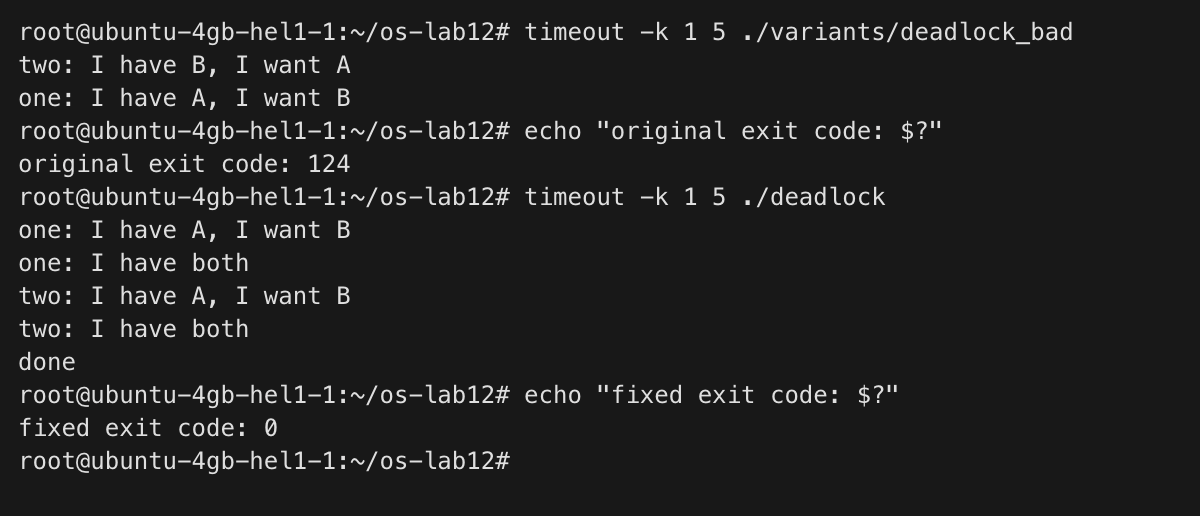
\includegraphics[width=\linewidth,height=0.67\textheight,keepaspectratio]{Lab12/evidence/screenshots/lab12-deadlock-fixed-terminal.png}
\end{minipage}\par\medskip

In this repeat run, thread two prints that it holds B and wants A, then
thread one prints that it holds A and wants B. The incorrect version
makes no further progress and the five-second timeout returns 124. The
fixed version prints both
{\ttfamily\fontsize{10}{12}\selectfont I have both} messages,
{\ttfamily\fontsize{10}{12}\selectfont done}, and exit code 0. Its
diagnostics correctly describe both threads acquiring A before B. The
reversed order of the first two diagnostic lines relative to the initial
saved run does not change the circular wait.

\subsubsection{Native Terminal evidence --- ten runs without
sleeps}\label{native-terminal-evidence-ten-runs-without-sleeps}

\par\medskip\noindent\begin{minipage}{\linewidth}\setstretch{1.0}
\captionof*{figure}{Figura 6. Native Terminal capture: absence of sleep calls, ten timeout results, and the first run’s opposite-lock diagnostics.}
\centering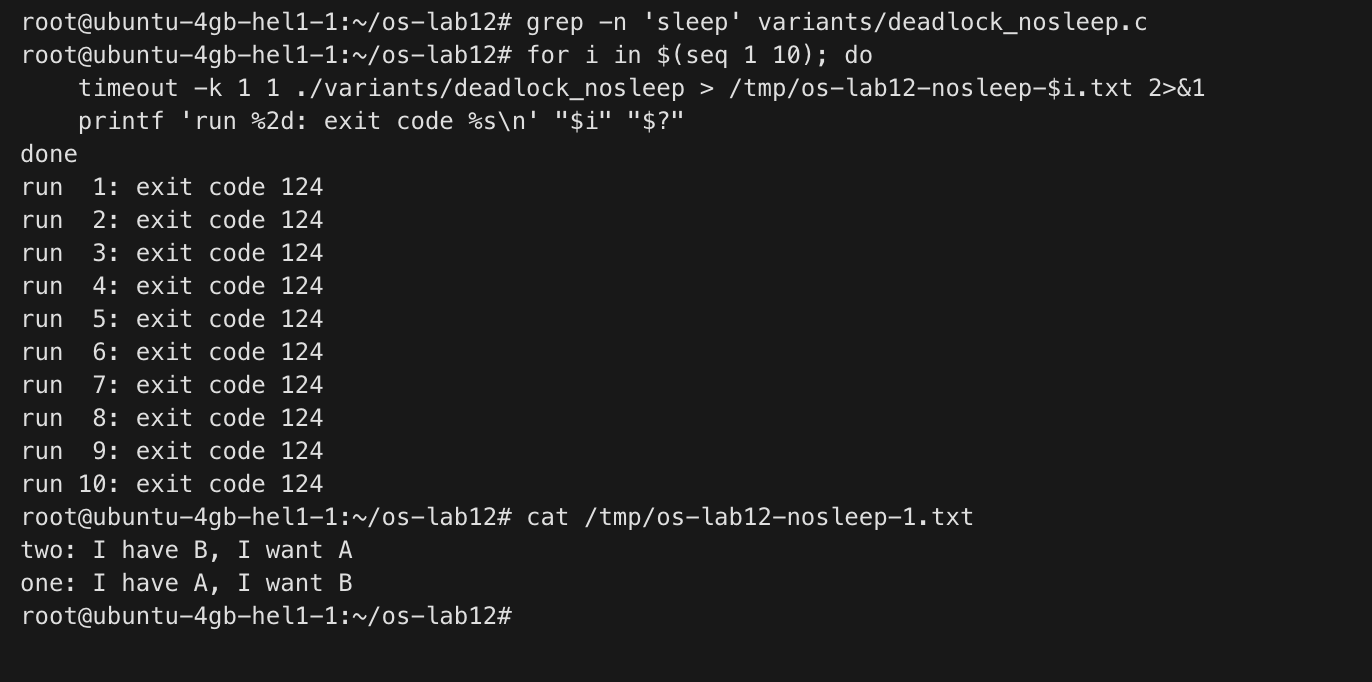
\includegraphics[width=\linewidth,height=0.67\textheight,keepaspectratio]{Lab12/evidence/screenshots/lab12-deadlock-nosleep-terminal.png}
\end{minipage}\par\medskip

The source search produces no matches for
{\ttfamily\fontsize{10}{12}\selectfont sleep}. All ten interactive
repetitions return code 124 under a one-second timeout. The saved first
repetition prints thread two holding B and requesting A, and thread one
holding A and requesting B. This repeat experiment therefore reproduces
the lock-order deadlock without the deliberate pauses. It does not
establish that every possible schedule must deadlock; removing the
sleeps leaves the circular-wait path intact.

\subsection{Reproduction and evidence}\label{reproduction-and-evidence}

Run {\ttfamily\fontsize{10}{12}\selectfont make clean all variants} on
Linux, then
{\ttfamily\fontsize{10}{12}\selectfont python3 run-experime\allowbreak{}nts.py}
to reproduce the experiments and checks. The runner overwrites its
evidence files with the new results. Deliberately incorrect programs are
always run with a timeout. The submitted source
{\ttfamily\fontsize{10}{12}\selectfont deadlock.c} is the fixed version.

\href{https://github.com/igortacu/OS/blob/main/Lab12/CAPTURES.md}{Terminal
capture commands} organize the live repetitions into readable blocks.
All six native Terminal screenshots are embedded above with captions and
observations. They document the interactive repeat runs; the initial
scripted measurements are retained separately in the text logs.

\par\noindent\begin{minipage}{\linewidth}

\section{Concluzie}\label{concluzie}

Bufferul păstrează ordinea și limitele de capacitate, iar variabila de
condiție cere re-verificarea stării după trezire. Ordinea comună A--B
permite terminarea celor două fire, în timp ce eliminarea pauzelor din
varianta greșită nu înlătură defectul de sincronizare.

\end{minipage}\par

\end{document}
